\documentclass[twoside]{book}

% Packages required by doxygen
\usepackage{calc}
\usepackage{doxygen}
\usepackage{graphicx}
\usepackage[utf8]{inputenc}
\usepackage{makeidx}
\usepackage{multicol}
\usepackage{multirow}
\usepackage{textcomp}
\usepackage[table]{xcolor}

% Font selection
\usepackage[T1]{fontenc}
\usepackage{mathptmx}
\usepackage[scaled=.90]{helvet}
\usepackage{courier}
\usepackage{amssymb}
\usepackage{sectsty}
\renewcommand{\familydefault}{\sfdefault}
\allsectionsfont{%
  \fontseries{bc}\selectfont%
  \color{darkgray}%
}
\renewcommand{\DoxyLabelFont}{%
  \fontseries{bc}\selectfont%
  \color{darkgray}%
}

% Page & text layout
\usepackage{geometry}
\geometry{%
  a4paper,%
  top=2.5cm,%
  bottom=2.5cm,%
  left=2.5cm,%
  right=2.5cm%
}
\tolerance=750
\hfuzz=15pt
\hbadness=750
\setlength{\emergencystretch}{15pt}
\setlength{\parindent}{0cm}
\setlength{\parskip}{0.2cm}
\makeatletter
\renewcommand{\paragraph}{%
  \@startsection{paragraph}{4}{0ex}{-1.0ex}{1.0ex}{%
    \normalfont\normalsize\bfseries\SS@parafont%
  }%
}
\renewcommand{\subparagraph}{%
  \@startsection{subparagraph}{5}{0ex}{-1.0ex}{1.0ex}{%
    \normalfont\normalsize\bfseries\SS@subparafont%
  }%
}
\makeatother

% Headers & footers
\usepackage{fancyhdr}
\pagestyle{fancyplain}
\fancyhead[LE]{\fancyplain{}{\bfseries\thepage}}
\fancyhead[CE]{\fancyplain{}{}}
\fancyhead[RE]{\fancyplain{}{\bfseries\leftmark}}
\fancyhead[LO]{\fancyplain{}{\bfseries\rightmark}}
\fancyhead[CO]{\fancyplain{}{}}
\fancyhead[RO]{\fancyplain{}{\bfseries\thepage}}
\fancyfoot[LE]{\fancyplain{}{}}
\fancyfoot[CE]{\fancyplain{}{}}
\fancyfoot[RE]{\fancyplain{}{\bfseries\scriptsize Generated on Thu Jan 30 2014 21\-:56\-:18 for Book Market by Doxygen }}
\fancyfoot[LO]{\fancyplain{}{\bfseries\scriptsize Generated on Thu Jan 30 2014 21\-:56\-:18 for Book Market by Doxygen }}
\fancyfoot[CO]{\fancyplain{}{}}
\fancyfoot[RO]{\fancyplain{}{}}
\renewcommand{\footrulewidth}{0.4pt}
\renewcommand{\chaptermark}[1]{%
  \markboth{#1}{}%
}
\renewcommand{\sectionmark}[1]{%
  \markright{\thesection\ #1}%
}

% Indices & bibliography
\usepackage{natbib}
\usepackage[titles]{tocloft}
\setcounter{tocdepth}{3}
\setcounter{secnumdepth}{5}
\makeindex

% Hyperlinks (required, but should be loaded last)
\usepackage{ifpdf}
\ifpdf
  \usepackage[pdftex,pagebackref=true]{hyperref}
\else
  \usepackage[ps2pdf,pagebackref=true]{hyperref}
\fi
\hypersetup{%
  colorlinks=true,%
  linkcolor=blue,%
  citecolor=blue,%
  unicode%
}

% Custom commands
\newcommand{\clearemptydoublepage}{%
  \newpage{\pagestyle{empty}\cleardoublepage}%
}


%===== C O N T E N T S =====

\begin{document}

% Titlepage & ToC
\hypersetup{pageanchor=false}
\pagenumbering{roman}
\begin{titlepage}
\vspace*{7cm}
\begin{center}%
{\Large Book Market }\\
\vspace*{1cm}
{\large Generated by Doxygen 1.8.5}\\
\vspace*{0.5cm}
{\small Thu Jan 30 2014 21:56:18}\\
\end{center}
\end{titlepage}
\clearemptydoublepage
\tableofcontents
\clearemptydoublepage
\pagenumbering{arabic}
\hypersetup{pageanchor=true}

%--- Begin generated contents ---
\chapter{Main Page}
\label{index}\hypertarget{index}{}\input{index}
\chapter{Hierarchical Index}
\section{Class Hierarchy}
This inheritance list is sorted roughly, but not completely, alphabetically\-:\begin{DoxyCompactList}
\item \contentsline{section}{com.\-lakehead.\-textbookmarket.\-Book}{\pageref{classcom_1_1lakehead_1_1textbookmarket_1_1_book}}{}
\item \contentsline{section}{com.\-lakehead.\-textbookmarket.\-Build\-Config}{\pageref{classcom_1_1lakehead_1_1textbookmarket_1_1_build_config}}{}
\item \contentsline{section}{com.\-lakehead.\-textbookmarket.\-Course}{\pageref{classcom_1_1lakehead_1_1textbookmarket_1_1_course}}{}
\item \contentsline{section}{com.\-lakehead.\-textbookmarket.\-Intent\-Integrator}{\pageref{classcom_1_1lakehead_1_1textbookmarket_1_1_intent_integrator}}{}
\item \contentsline{section}{com.\-lakehead.\-textbookmarket.\-Intent\-Result}{\pageref{classcom_1_1lakehead_1_1textbookmarket_1_1_intent_result}}{}
\item \contentsline{section}{com.\-lakehead.\-textbookmarket.\-Listing}{\pageref{classcom_1_1lakehead_1_1textbookmarket_1_1_listing}}{}
\item \contentsline{section}{com.\-lakehead.\-textbookmarket.\-On\-Task\-Completed}{\pageref{interfacecom_1_1lakehead_1_1textbookmarket_1_1_on_task_completed}}{}
\begin{DoxyCompactList}
\item \contentsline{section}{com.\-lakehead.\-textbookmarket.\-Books\-Fragment}{\pageref{classcom_1_1lakehead_1_1textbookmarket_1_1_books_fragment}}{}
\end{DoxyCompactList}
\item \contentsline{section}{com.\-lakehead.\-textbookmarket.\-R}{\pageref{classcom_1_1lakehead_1_1textbookmarket_1_1_r}}{}
\item Tab\-Listener\begin{DoxyCompactList}
\item \contentsline{section}{com.\-lakehead.\-textbookmarket.\-Main\-Activity}{\pageref{classcom_1_1lakehead_1_1textbookmarket_1_1_main_activity}}{}
\end{DoxyCompactList}
\item Activity\begin{DoxyCompactList}
\item \contentsline{section}{com.\-lakehead.\-textbookmarket.\-Add\-Listing\-Activity}{\pageref{classcom_1_1lakehead_1_1textbookmarket_1_1_add_listing_activity}}{}
\item \contentsline{section}{com.\-lakehead.\-textbookmarket.\-Login\-Activity}{\pageref{classcom_1_1lakehead_1_1textbookmarket_1_1_login_activity}}{}
\item \contentsline{section}{com.\-lakehead.\-textbookmarket.\-Register\-Activity}{\pageref{classcom_1_1lakehead_1_1textbookmarket_1_1_register_activity}}{}
\end{DoxyCompactList}
\item Array\-Adapter\begin{DoxyCompactList}
\item \contentsline{section}{com.\-lakehead.\-textbookmarket.\-Book\-Array\-Adapter}{\pageref{classcom_1_1lakehead_1_1textbookmarket_1_1_book_array_adapter}}{}
\item \contentsline{section}{com.\-lakehead.\-textbookmarket.\-Course\-Array\-Adapter}{\pageref{classcom_1_1lakehead_1_1textbookmarket_1_1_course_array_adapter}}{}
\item \contentsline{section}{com.\-lakehead.\-textbookmarket.\-Listing\-Array\-Adapter}{\pageref{classcom_1_1lakehead_1_1textbookmarket_1_1_listing_array_adapter}}{}
\end{DoxyCompactList}
\item Fragment\begin{DoxyCompactList}
\item \contentsline{section}{com.\-lakehead.\-textbookmarket.\-Books\-Fragment}{\pageref{classcom_1_1lakehead_1_1textbookmarket_1_1_books_fragment}}{}
\item \contentsline{section}{com.\-lakehead.\-textbookmarket.\-Courses\-Fragment}{\pageref{classcom_1_1lakehead_1_1textbookmarket_1_1_courses_fragment}}{}
\item \contentsline{section}{com.\-lakehead.\-textbookmarket.\-Listings\-Fragment}{\pageref{classcom_1_1lakehead_1_1textbookmarket_1_1_listings_fragment}}{}
\end{DoxyCompactList}
\item Fragment\-Activity\begin{DoxyCompactList}
\item \contentsline{section}{com.\-lakehead.\-textbookmarket.\-Main\-Activity}{\pageref{classcom_1_1lakehead_1_1textbookmarket_1_1_main_activity}}{}
\end{DoxyCompactList}
\item Fragment\-Pager\-Adapter\begin{DoxyCompactList}
\item \contentsline{section}{com.\-lakehead.\-textbookmarket.\-Tabs\-Pager\-Adapter}{\pageref{classcom_1_1lakehead_1_1textbookmarket_1_1_tabs_pager_adapter}}{}
\end{DoxyCompactList}
\item Preference\-Activity\begin{DoxyCompactList}
\item \contentsline{section}{com.\-lakehead.\-textbookmarket.\-Settings\-Activity}{\pageref{classcom_1_1lakehead_1_1textbookmarket_1_1_settings_activity}}{}
\end{DoxyCompactList}
\end{DoxyCompactList}

\chapter{Class Index}
\section{Class List}
Here are the classes, structs, unions and interfaces with brief descriptions\-:\begin{DoxyCompactList}
\item\contentsline{section}{\hyperlink{classcom_1_1lakehead_1_1textbookmarket_1_1_add_listing_activity}{com.\-lakehead.\-textbookmarket.\-Add\-Listing\-Activity} \\*Class that handles I\-S\-B\-N Lookup }{\pageref{classcom_1_1lakehead_1_1textbookmarket_1_1_add_listing_activity}}{}
\item\contentsline{section}{\hyperlink{classcom_1_1lakehead_1_1textbookmarket_1_1_book}{com.\-lakehead.\-textbookmarket.\-Book} \\*Created by Master on 2/10/14 }{\pageref{classcom_1_1lakehead_1_1textbookmarket_1_1_book}}{}
\item\contentsline{section}{\hyperlink{classcom_1_1lakehead_1_1textbookmarket_1_1_book_array_adapter}{com.\-lakehead.\-textbookmarket.\-Book\-Array\-Adapter} \\*Adapter used to fill a List\-View with data from a \hyperlink{classcom_1_1lakehead_1_1textbookmarket_1_1_book}{Book} object }{\pageref{classcom_1_1lakehead_1_1textbookmarket_1_1_book_array_adapter}}{}
\item\contentsline{section}{\hyperlink{classcom_1_1lakehead_1_1textbookmarket_1_1_books_fragment}{com.\-lakehead.\-textbookmarket.\-Books\-Fragment} \\*The fragment used in the \char`\"{}\-Books\char`\"{} tab of \hyperlink{classcom_1_1lakehead_1_1textbookmarket_1_1_main_activity}{Main\-Activity} }{\pageref{classcom_1_1lakehead_1_1textbookmarket_1_1_books_fragment}}{}
\item\contentsline{section}{\hyperlink{classcom_1_1lakehead_1_1textbookmarket_1_1_build_config}{com.\-lakehead.\-textbookmarket.\-Build\-Config} }{\pageref{classcom_1_1lakehead_1_1textbookmarket_1_1_build_config}}{}
\item\contentsline{section}{\hyperlink{classcom_1_1lakehead_1_1textbookmarket_1_1_course}{com.\-lakehead.\-textbookmarket.\-Course} \\*Created by Master on 2/17/14 }{\pageref{classcom_1_1lakehead_1_1textbookmarket_1_1_course}}{}
\item\contentsline{section}{\hyperlink{classcom_1_1lakehead_1_1textbookmarket_1_1_course_array_adapter}{com.\-lakehead.\-textbookmarket.\-Course\-Array\-Adapter} \\*The adapter used to populate the list view for the courses fragment }{\pageref{classcom_1_1lakehead_1_1textbookmarket_1_1_course_array_adapter}}{}
\item\contentsline{section}{\hyperlink{classcom_1_1lakehead_1_1textbookmarket_1_1_courses_fragment}{com.\-lakehead.\-textbookmarket.\-Courses\-Fragment} \\*The fragment used in the \char`\"{}\-Books\char`\"{} tab of \hyperlink{classcom_1_1lakehead_1_1textbookmarket_1_1_main_activity}{Main\-Activity} }{\pageref{classcom_1_1lakehead_1_1textbookmarket_1_1_courses_fragment}}{}
\item\contentsline{section}{\hyperlink{classcom_1_1lakehead_1_1textbookmarket_1_1_intent_integrator}{com.\-lakehead.\-textbookmarket.\-Intent\-Integrator} \\*Class handling the launching of the scanner }{\pageref{classcom_1_1lakehead_1_1textbookmarket_1_1_intent_integrator}}{}
\item\contentsline{section}{\hyperlink{classcom_1_1lakehead_1_1textbookmarket_1_1_intent_result}{com.\-lakehead.\-textbookmarket.\-Intent\-Result} \\*Encapsulates the result of a barcode scan invoked through \hyperlink{classcom_1_1lakehead_1_1textbookmarket_1_1_intent_integrator}{Intent\-Integrator} }{\pageref{classcom_1_1lakehead_1_1textbookmarket_1_1_intent_result}}{}
\item\contentsline{section}{\hyperlink{classcom_1_1lakehead_1_1textbookmarket_1_1_listing}{com.\-lakehead.\-textbookmarket.\-Listing} \\*Class holding all listing information }{\pageref{classcom_1_1lakehead_1_1textbookmarket_1_1_listing}}{}
\item\contentsline{section}{\hyperlink{classcom_1_1lakehead_1_1textbookmarket_1_1_listing_array_adapter}{com.\-lakehead.\-textbookmarket.\-Listing\-Array\-Adapter} \\*Created by Master on 2/17/14 }{\pageref{classcom_1_1lakehead_1_1textbookmarket_1_1_listing_array_adapter}}{}
\item\contentsline{section}{\hyperlink{classcom_1_1lakehead_1_1textbookmarket_1_1_listings_fragment}{com.\-lakehead.\-textbookmarket.\-Listings\-Fragment} \\*The fragment used in the \char`\"{}\-Listings\char`\"{} tab of \hyperlink{classcom_1_1lakehead_1_1textbookmarket_1_1_main_activity}{Main\-Activity} }{\pageref{classcom_1_1lakehead_1_1textbookmarket_1_1_listings_fragment}}{}
\item\contentsline{section}{\hyperlink{classcom_1_1lakehead_1_1textbookmarket_1_1_login_activity}{com.\-lakehead.\-textbookmarket.\-Login\-Activity} \\*This \hyperlink{interfacecom_1_1lakehead_1_1textbookmarket_1_1_on_task_completed}{On\-Task\-Completed} is an interface that Activities receiving callbacks from async tasks should implement }{\pageref{classcom_1_1lakehead_1_1textbookmarket_1_1_login_activity}}{}
\item\contentsline{section}{\hyperlink{classcom_1_1lakehead_1_1textbookmarket_1_1_main_activity}{com.\-lakehead.\-textbookmarket.\-Main\-Activity} \\*Primary Activity Holding the tabs managed by \hyperlink{classcom_1_1lakehead_1_1textbookmarket_1_1_tabs_pager_adapter}{Tabs\-Pager\-Adapter} , it also handles the action bar }{\pageref{classcom_1_1lakehead_1_1textbookmarket_1_1_main_activity}}{}
\item\contentsline{section}{\hyperlink{interfacecom_1_1lakehead_1_1textbookmarket_1_1_on_task_completed}{com.\-lakehead.\-textbookmarket.\-On\-Task\-Completed} \\*A simple interface used to ensure objects implement a callback function that can be used with Async\-Tasks }{\pageref{interfacecom_1_1lakehead_1_1textbookmarket_1_1_on_task_completed}}{}
\item\contentsline{section}{\hyperlink{classcom_1_1lakehead_1_1textbookmarket_1_1_r}{com.\-lakehead.\-textbookmarket.\-R} }{\pageref{classcom_1_1lakehead_1_1textbookmarket_1_1_r}}{}
\item\contentsline{section}{\hyperlink{classcom_1_1lakehead_1_1textbookmarket_1_1_register_activity}{com.\-lakehead.\-textbookmarket.\-Register\-Activity} \\*Activity used for user Registration }{\pageref{classcom_1_1lakehead_1_1textbookmarket_1_1_register_activity}}{}
\item\contentsline{section}{\hyperlink{classcom_1_1lakehead_1_1textbookmarket_1_1_settings_activity}{com.\-lakehead.\-textbookmarket.\-Settings\-Activity} \\*A \hyperlink{}{Preference\-Activity} that presents a set of application settings }{\pageref{classcom_1_1lakehead_1_1textbookmarket_1_1_settings_activity}}{}
\item\contentsline{section}{\hyperlink{classcom_1_1lakehead_1_1textbookmarket_1_1_tabs_pager_adapter}{com.\-lakehead.\-textbookmarket.\-Tabs\-Pager\-Adapter} \\*Handles the logic of switching between tabs }{\pageref{classcom_1_1lakehead_1_1textbookmarket_1_1_tabs_pager_adapter}}{}
\end{DoxyCompactList}

\chapter{Class Documentation}
\hypertarget{classcom_1_1lakehead_1_1textbookmarket_1_1_main_activity}{\section{com.\-lakehead.\-textbookmarket.\-Main\-Activity Class Reference}
\label{classcom_1_1lakehead_1_1textbookmarket_1_1_main_activity}\index{com.\-lakehead.\-textbookmarket.\-Main\-Activity@{com.\-lakehead.\-textbookmarket.\-Main\-Activity}}
}
Inheritance diagram for com.\-lakehead.\-textbookmarket.\-Main\-Activity\-:\begin{figure}[H]
\begin{center}
\leavevmode
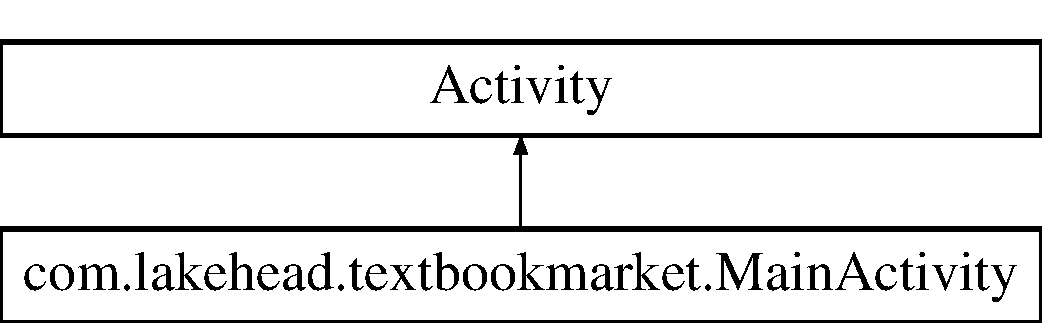
\includegraphics[height=2.000000cm]{classcom_1_1lakehead_1_1textbookmarket_1_1_main_activity}
\end{center}
\end{figure}
\subsection*{Classes}
\begin{DoxyCompactItemize}
\item 
class {\bfseries Placeholder\-Fragment}
\begin{DoxyCompactList}\small\item\em A placeholder fragment containing a simple view. \end{DoxyCompactList}\end{DoxyCompactItemize}
\subsection*{Public Member Functions}
\begin{DoxyCompactItemize}
\item 
\hypertarget{classcom_1_1lakehead_1_1textbookmarket_1_1_main_activity_a42aad44340fa4dd995cca807512be2bf}{boolean {\bfseries on\-Create\-Options\-Menu} (Menu menu)}\label{classcom_1_1lakehead_1_1textbookmarket_1_1_main_activity_a42aad44340fa4dd995cca807512be2bf}

\item 
\hypertarget{classcom_1_1lakehead_1_1textbookmarket_1_1_main_activity_a9e9ecfdbbbb7ad1d0ecec7ba405701a6}{boolean {\bfseries on\-Options\-Item\-Selected} (Menu\-Item item)}\label{classcom_1_1lakehead_1_1textbookmarket_1_1_main_activity_a9e9ecfdbbbb7ad1d0ecec7ba405701a6}

\end{DoxyCompactItemize}
\subsection*{Protected Member Functions}
\begin{DoxyCompactItemize}
\item 
\hypertarget{classcom_1_1lakehead_1_1textbookmarket_1_1_main_activity_ab5dc3cecf5c66f0c5e7ab996b6143fe4}{void {\bfseries on\-Create} (Bundle saved\-Instance\-State)}\label{classcom_1_1lakehead_1_1textbookmarket_1_1_main_activity_ab5dc3cecf5c66f0c5e7ab996b6143fe4}

\end{DoxyCompactItemize}


\subsection{Detailed Description}


Definition at line 14 of file Main\-Activity.\-java.



The documentation for this class was generated from the following file\-:\begin{DoxyCompactItemize}
\item 
C\-:/\-Users/\-Master/\-Documents/\-Git\-Hub/\-C\-S4431-\/android/\-Textbook\-Market/src/main/java/com/lakehead/textbookmarket/Main\-Activity.\-java\end{DoxyCompactItemize}

%--- End generated contents ---

% Index
\newpage
\phantomsection
\addcontentsline{toc}{part}{Index}
\printindex

\end{document}
